\newpage
\subsection{Emitters}
\label{sec:emitters}
Mitsuba supports a wide range of emitters/light sources, which can be classified
into two main categories: emitters which are located somewhere within the scene, and emitters
that \emph{surround} the scene to simulate a distant environment. An overview of the available
types is shown below:
\begin{figure}[h!]
\centering
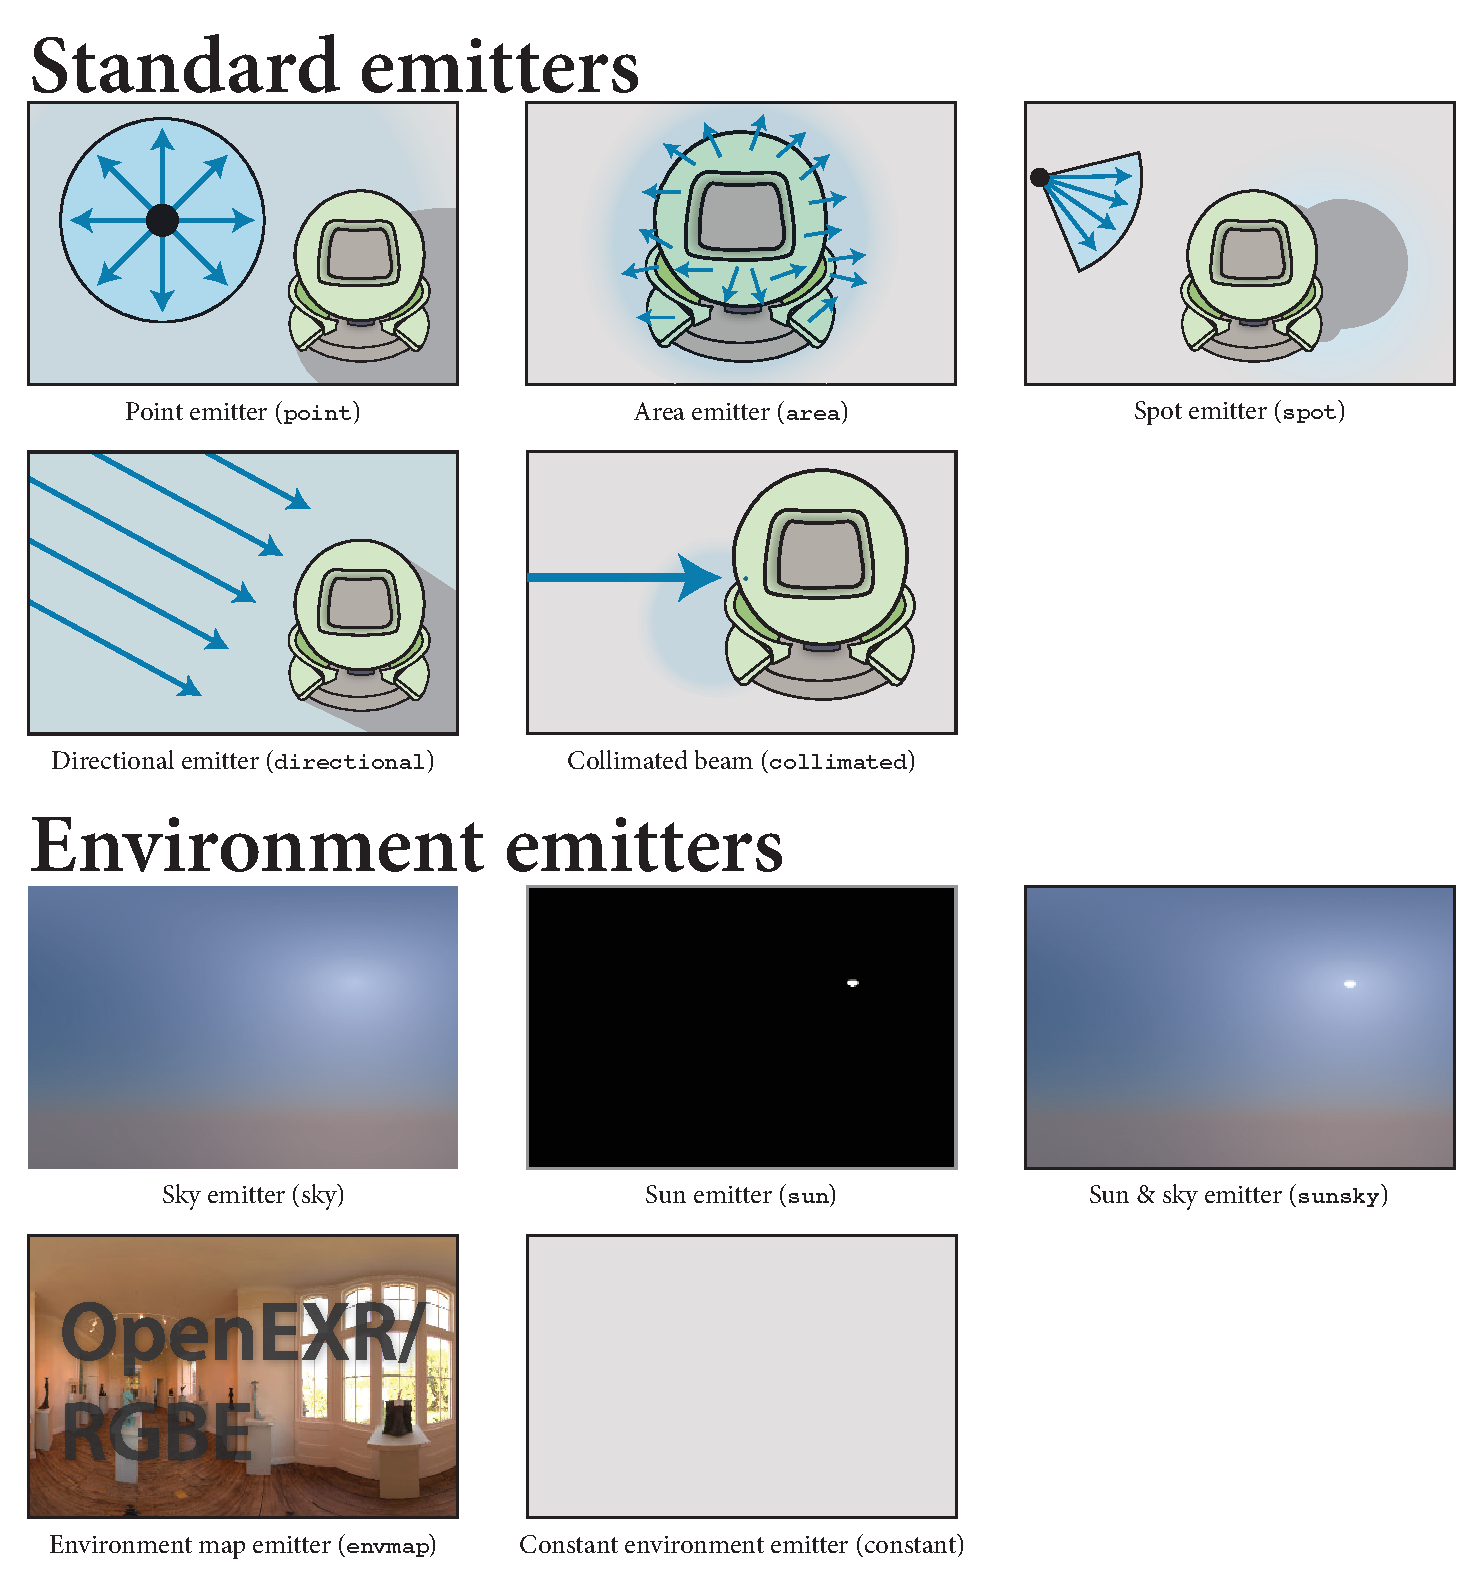
\includegraphics[width=15.5cm]{images/emitter_overview.pdf}
\caption{
    Schematic overview of the most important emitters in Mitsuba.
    The arrows indicate the directional distribution of light.
}
\end{figure}
